\documentclass[conference]{IEEEtran}
\IEEEoverridecommandlockouts
\usepackage{amsmath} % para ambientes e comandos matemáticos
\usepackage{cite}
\usepackage{amsmath,amssymb,amsfonts}
\usepackage{algorithmic}
\usepackage{graphicx}
\usepackage{textcomp}
\usepackage{xcolor}
\def\BibTeX{{\rm B\kern-.05em{\sc i\kern-.025em b}\kern-.08em
    T\kern-.1667em\lower.7ex\hbox{E}\kern-.125emX}}
\begin{document}

\title{Avaliação Comparativa de Classificadores : Um Tradeoff entre Custo Temporal e Performance\\
\thanks{Identify applicable funding agency here. If none, delete this.}
}

\author{\IEEEauthorblockN{Arthur Felipe Reis Souza.}
\IEEEauthorblockA{\textit{Departamento de Engenharia Elétrica} \\
\textit{Universidade Federal de Minas Gerais}\\
Belo Horizonte, Brasil \\
arthurfreisouza@gmail.com}
\and
\IEEEauthorblockN{Antônio de Pádua Braga}
\IEEEauthorblockA{\textit{Departamento de Engenharia Elétrica} \\
\textit{Universidade Federal de Minas Gerais}\\
Belo Horizonte, Brasil \\
apbraga@cpdee.ufmg.br}
}

\maketitle

\begin{abstract}
    Este artigo tem por objetivo analisar o custo temporal de diversos algoritmos de machine learning, com o intuito de identificar algoritos que executam mais rápido em uma certa base de dados, sem comprometer significativamente o desempenho. Embora diferentes algoritmos possam atingir resultados similares em termos de precisão sobre um mesmo conjunto de dados, eles podem diferir significativamente quando se trata de tempo de execução. Portanto, é crucial compreender as circunstâncias ideais para a aplicação de cada algoritmo, visando economizar tempo e energia, ao mesmo tempo em que se mantém uma alta eficiência.
    
    Para a análise, foram utilizados dois conjuntos de dados de classificação: um conjunto de dados simples do "Titanic" e um conjunto de dados mais extenso do Santander. Esses conjuntos de dados foram utilizados para treinar quatro classificadores: um KNN, um classificador Bayesiano e duas redes neurais perceptron multicamadas (MLP) com otimizadores diferentes. Os resultados dos tempos de treinamento e teste, bem como as acurácias, foram registrados em uma tabela e posteriormente analisadas.
\end{abstract}

\begin{IEEEkeywords}
component, formatting, style, styling, insert
\end{IEEEkeywords}

\section{Introduction}

Com os avanços tecnológicos e matemáticos, que possibilitaram a aplicação de algoritmos de aprendizado de máquina, torna-se essencial que os desenvolvedores analisem cuidadosamente a relação custo-benefício de cada algoritmo, levando em conta o significativo poder de processamento envolvido. Isso ocorre porque alguns algoritmos podem alcançar desempenhos semelhantes, mas com custos temporais e energéticos consideravelmente menores. Assim, o objetivo deste artigo é avaliar a aplicação de quatro diferentes algoritmos de machine learning em duas bases de dados distintas, examinando como cada algoritmo se ajusta a cada uma dessas bases.

Para a análise do desempenho desses algoritmos, foram utilizadas duas bases de dados de classificação, ambas obtidas diretamente de competições no Kaggle. A primeira base de dados é do "Titanic", contendo informações e características dos passageiros a bordo, com o objetivo de prever se uma pessoa com determinados atributos sobreviveu ao naufrágio. A segunda base de dados é da competição "Santander" do Kaggle, caracterizada por um grande volume de dados com diversas características ocultas. O objetivo é desenvolver um classificador para prever se um cliente realizará uma transferência no futuro com base nas informações disponíveis.

Após obter as bases de dados no kaggle e realizar a leitura dos dados, realizou-se um preprocessamento para detectar potenciais fatores que poderiam afetar a eficiência dos classificadores, como valores não representativos e multicolinearidade. Em seguida, aplicaram-se quatro classificadores distintos: KNN, classificador Bayesiano e duas arquiteturas diferentes de redes neurais de múltiplas camadas. Uma das arquiteturas utilizou o otimizador Adaptive Moment Estimation (ADAM), enquanto a outra emprega o Stochastic Gradient Descent (SGD). 

Os hiperparâmetros de cada modelo foram obtidos através da técnica de GridSearch, onde diversas combinações são testadas em um grid pré-definido. A combinação de hiperparâmetros que resultou na melhor performance, de acordo com a métrica escolhida para o problema, foi selecionada. Cada modelo ótimo é então criado, e testado com a técnica de cross-validation nas mesmas amostras do Grid, resultando então em uma acurácia média do modelo sobre os dados de treino. Em seguida, o modelo foi validado com os dados de validação e o valor de threshold que otimizou a acurácia foi obtido com a curva ROC, tendo sido definido como o threshold do modelo.

Por fim, as combinações de hiperparâmetros resultantes, o tempo de treinamento, o tempo de teste e a performance de cada modelo foram registrados em uma tabela, para serem comparados e analisados.

\section{Research Methodology}

\subsection{Pre-processing Data}

O pré-processamento de ambos os datasets envolveu a remoção de colunas com baixa representatividade e valores nominais. Para tratar as colunas com valores faltantes, utilizou-se o algoritmo KNN Imputer. Este algoritmo, baseado no método KNN (K-Nearest Neighbors), preenche valores binários com a moda e valores contínuos com a média dos K vizinhos mais próximos[9].

\subsection{Training and Validation}

O treinamento envolveu a aplicação de um GridSearch para otimizar os hiperparâmetros dos quatro modelos. Posteriormente, calcularam-se as acurácias médias de cada um deles. Por fim, os thresholds de cada modelo foram ajustados para maximizar a acurácia na curva ROC (Receiver Operating Characteristic Curve)[6][7].

\subsection{Results}

Como resultado, teremos a curva ROC, que mostra o ponto onde o threshold proporciona a melhor acurácia do classificador, além de uma tabela que destaca os desempenhos e características de cada modelo[6][7].

\section{Literature Study}

\subsection{Receiver Operating Characteristic}

A curva ROC (Receiver Operating Characteristic) é uma representação gráfica da performance de um classificador binário enquanto se varia o threshold ao longo do intervalo [0, 1]. A ideia é que, para cada valor do threshold, obtêm-se os valores da sensibilidade (True positive rate) e da especificidade (1 - False positive rate). Uma métrica comum para avaliar classificadores é a área abaixo da curva ROC, também conhecida como AUC (Area Under the Curve). Quanto maior o valor da AUC, melhor é de se esperar o desempenho do classificador.


\subsection{Ridge Regression (L2 Regularization)}

A regularização Ridge Regression envolve a inclusão de um termo \(\lambda \) na função de custo, que será ponderado pelo valor de cada peso. Esse termo penaliza os parâmetros do modelo, ajudando a controlar sua complexidade e a reduzir o overfitting.

A função de custo regularizada com Ridge Regression é dada por:
\[ J(\mathbf{w}) = \frac{1}{2m} \sum_{i=1}^{m} (h_{\mathbf{w}}(\mathbf{x}^{(i)}) - y^{(i)})^2 + \frac{\lambda}{2m} \sum_{j=1}^{n} w_j^2 \]

onde:
\begin{itemize}
    \item \( J(\mathbf{w}) \): Função de custo regularizada com Ridge Regression.
    \item \( \mathbf{w} \): Vetor de pesos do modelo.
    \item \( m \): Número de exemplos de treinamento.
    \item \( h_{\mathbf{w}}(\mathbf{x}^{(i)}) \): Predição do modelo para o exemplo \( \mathbf{x}^{(i)} \).
    \item \( y^{(i)} \): Resposta verdadeira para o exemplo \( \mathbf{x}^{(i)} \).
    \item \( \lambda \): Parâmetro de regularização que controla a força da penalização L2.
    \item \( n \): Número de pesos no vetor \( \mathbf{w} \).
    \item \( w_j \): \( j \)-ésimo peso no vetor \( \mathbf{w} \).
\end{itemize}


\subsection{Naive Bayes Algorithm}

O classificador Naive Bayes baseia-se na regra de Bayes e na independência das variáveis de entrada (correlação nula entre os atributos de entrada), para estimar a probabilidade a posteriori de uma amostra pertencer a uma classe, utilizando uma função de verossimilhança que é multiplicada pela probabilidade a priori da classe[1][2][5]. A amostra é então atribuída à classe com a maior probabilidade a posteriori. A Regra de Bayes é dada pela equação :

\[
P(C|x) = \frac{P(x|C) \cdot P(C)}{P(x)} \quad \text{, onde:}
\]
\begin{itemize}
    \item \( P(C|x) \) é a probabilidade posterior de \( C \) dado a ocorrência de \( x \),
    \item \( P(x|C) \) é o "likelihood" de \( x \) dado \( C \) ou  função de verossimilhança,
    \item \( P(C) \) é a probabilidade a prior da classe \( C \) ocorrer,
    \item \( P(x) \) é a evidência \( x \) ou a probabilidade de x ocorrer.
\end{itemize}

\vspace{10pt}

Para ser um classificador eficaz, o Naive Bayes requer amostras que sejam representativas e não apresentem sobreposição significativa entre as classes. Quando há uma grande sobreposição entre as classes, as funções de densidade também se sobrepõem, o que pode resultar em um desempenho inferior do classificador[1].

\subsection{K-Nearest Neighboors}

O KNN (K-Nearest Neighbors) é um classificador que se baseia nos K vizinhos mais próximos. Ele opera calculando a distância, baseado em alguma métrica específica, entre todos os pontos de treinamento e a amostra de teste. Há várias métricas de distância possíveis, sendo a distância de Minkowski a mais geral. Essa métrica contém um hiperparâmetro r que pode ser aprendido e ajustado no processo de treinamento.

\[
D(\mathbf{p}, \mathbf{q}) = \left( \sum_{i=1}^{n} |p_i - q_i|^r \right)^{1/r}
\]

onde \( \mathbf{p} = (p_1, p_2, \ldots, p_n) \) e \( \mathbf{q} = (q_1, q_2, \ldots, q_n) \) são vetores de entrada, e \( r \) é um parâmetro que controla a ordem da distância Minkowski.

Pode se observar que, quando r = 1 a métrica de Minkowski se igua-la a métrica de Manhattan. E quando r = 2 a métrica de Minkowski se igua-la a métrica Euclideana.

Após todas as distâncias serem calculadas e ordenadas, o modelo classifica a amostra de teste com base na moda (mais frequente) das classes das K amostras de treino mais próximas. Para problemas de regressão, o KNN utiliza a média dos valores das K amostras mais próximas.

A métrica de distância utilizada no modelo foi a distância Euclideana, equivalente a ter o r = 2, na equação da métrica de Minkowski.

\subsection{Multi-Layer Perceptron}

As redes neurais do tipo Multi Layer Perceptron (MLP) são conhecidas como aproximadoras universais de funções e são amplamente utilizadas em tarefas de regressão, classificação e previsão. Esses modelos podem ser configurados de diversas maneiras, utilizando diferentes conjuntos de hiperparâmetros. Todos eles empregam o algoritmo de backpropagation, utilizado para retropropagar o erro através das camadas da rede e realizar o ajuste dos pesos[1].

No desenvolvimento de um modelo Perceptron de Múltiplas Camadas, é crucial empregar técnicas de regularização para mitigar o overfitting. Esse fenômeno ocorre quando o modelo não apenas aprende a função geradora dos dados, mas também os ruídos presentes nos dados de entrada. Isso se reflete em um erro baixo nos dados de treino, mas um erro maior nos dados de teste. Para combater o overfitting, são empregadas técnicas de regularização projetadas para promover um aprendizado mais generalizado do modelo. A técnica de regularização utilizada e que visa controlar a complexidade do modelo é a Ridge Regression (L2 Regularization).

Durante a fase de treinamento, as entradas da rede são propagadas para frente camada por camada e linearizadas até a camada final, resultando em uma saída ŷ. Uma função de custo J é então utilizada para medir a discrepância entre a saída ŷ prevista pela rede e a saída y real. O objetivo do treinamento das redes neurais de múltiplas camadas é minimizar essa função de custo J, ajustando os parâmetros da rede de forma a aproximar ao máximo a saída ŷ da saída desejada y.

Existem várias abordagens para minimizar a função de custo, e a velocidade de convergência depende das características arquiteturais da rede, como funções de ativação, número de camadas e profundidade. Para acelerar esse processo de convergência, diversos algoritmos de otimização foram desenvolvidos, introduzindo características como taxa de aprendizado adaptativa e a inclusão de termos de momentum. Serão utilizados dois otimizadores, o Stochastic Gradient Descent (SGD) e o Adaptive Moment Estimation (ADAM).

\vspace{10pt}

\subsubsection{Stochastic Gradient Descent}

O Stochastic Gradient Descent (SGD) é um otimizador baseado no gradiente descendente, mas com uma abordagem diferente do gradiente descendente convencional. Enquanto o gradiente descendente comum atualiza os pesos considerando todas as entradas da rede, o SGD opera selecionando aleatoriamente uma entrada do conjunto de dados para calcular o gradiente usando o algoritmo de retropropagação de erros (backpropagation) e atualizar os parâmetros da rede[4].

Essa abordagem torna o SGD mais rápido em comparação com o gradiente descendente convencional, pois não calcula o gradiente e realiza a retropropagação para todas as entradas do conjunto de dados. Em vez disso, ele usa mini-batches estocásticos, o que proporciona uma eficiência computacional significativa, especialmente em conjuntos de dados grandes.

\[
\theta_{t+1} = \theta_t - \eta \nabla_{\theta} \mathcal{L}(\theta_t; x_i, y_i)
\]
onde:
\begin{itemize}
    \item \( \theta_t \) são os parâmetros dada a entrada no tempo \( t \),
    \item \( \eta \) é a taxa de aprendizado,
    \item \( \nabla_{\theta} \mathcal{L}(\theta_t; x_i, y_i) \) é o gradiente da função de perda \( \mathcal{L} \) em relação aos parâmetros \( \theta \) no ponto \( (\theta_t, x_i, y_i) \).
\end{itemize}

\vspace{10pt}
Este processo é repetido para cada mini-batch ou amostra aleatória \( (x_i, y_i) \) do conjunto de dados durante o treinamento do modelo. Um mini-batch é um subconjunto de um conjunto principal de amostras que foram selecionadas aleatoriamente para resultar na atualização dos pesos de uma rede neural.
\vspace{10pt}

\subsubsection{adaptive Moment Estimation}

O otimizador Adaptive Moment Estimation (ADAM) combina características de dois otimizadores distintos. Inclui características herdadas do RMSprop, e também do Stochastic Gradient Descent With Momentum.

O RMSprop ajusta a taxa de aprendizado \( \alpha \) adaptativamente ao invés de mantê-la constante ao longo do tempo. A nova taxa de aprendizado é calculada dividindo-se o a mesma por uma média móvel dos gradientes anteriores, ou seja, utiliza um ponderamento de gradientes anteriores para atualizar a taxa de aprendizado atual. Essa mudança constante de \( \alpha \) traz a vantagem de eliminar a necessidade de ajustar manualmente esse hiperparâmetro[4][8].

As equações de atualização dos pesos usando o otimizador RMSprop são:

\begin{align*}
v_{dw} & = \beta_{2} v_{dw} + (1 - \beta_{2}) (dw)^2 \\
w & = w - \alpha \frac{dw}{\sqrt{v_{dw} + \varepsilon}}
\end{align*}
onde:
\begin{itemize}
    \item \( w \) são os pesos a serem atualizados,
    \item \( dw \) é o gradiente do erro com respeito a \( w \),
    \item \( v_{dw} \) é a média exponencialmente decrescente dos quadrados dos gradientes,
    \item \( \alpha \) é a taxa de aprendizado,
    \item \( \beta_{2} \) é o fator de decaimento para a média exponencial dos quadrados dos gradientes,
    \item \( \varepsilon \) é um termo pequeno para evitar a divisão por zero.
\end{itemize}

O otimizador ADAM também incorpora um termo de momentum, que utiliza as informações dos gradientes anteriores na atualização dos pesos. Os gradientes passados, adicionados nas equações de atualização dos pesos atuais, são ponderados por um hiperparâmetro \( \beta_{2} \), conhecido como termo de momentum. A adição desses gradientes passados acelera a atualização dos pesos. No entanto, devido a essa aceleração, há um risco maior de ultrapassar mínimos locais e não convergir adequadamente.

As equações de atualização dos pesos usando o otimizador Momentum são:
\begin{align*}
m_{dw} & = \beta_{1} m_{dw} + (1 - \beta_{1}) dw \\
w & = w - \alpha m_{dw}
\end{align*}
onde:
\begin{itemize}
    \item \( w \) são os pesos a serem atualizados,
    \item \( dw \) é o gradiente do erro com respeito a \( w \),
    \item \( m_{dw} \) é o termo de momento que acumula o gradiente ao longo das iterações,
    \item \( \alpha \) é a taxa de aprendizado,
    \item \( \beta_{1} \) é o parâmetro de momento que controla a contribuição do momento anterior.
\end{itemize}

Portanto, o otimizador ADAM se baseia neses dois otimizadores anteriores para atualizar os parâmetros da rede. Sendo assim, a rede é adicionada de dois hiperparâmetros \( \beta_{1} \) e \( \beta_{2} \). Os valores desses hiperparâmetros pode ser encontrados através de técnicas de Grid, mas eles são comumente postos como : \( \beta_{1} \) = 0.9 , e \( \beta_{2} \) = 0.999.

\section{Results and discussions}

Após treinar a rede e obter os melhores hiperparâmetros com o GridSearch, foram obtidas as seguintes curvas ROC para o dataset do Titanic : 

\subsection{Titanic}

\vspace{20pt}

\begin{figure}[htbp]
\centerline{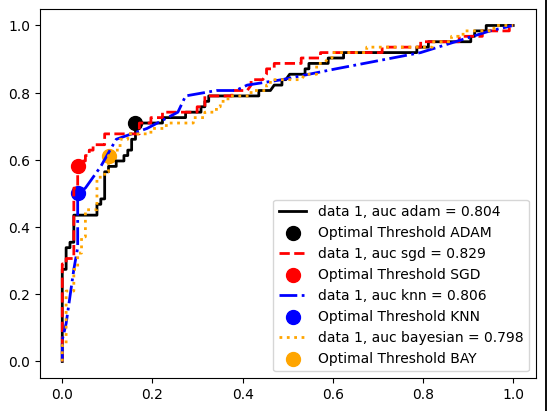
\includegraphics[width=0.25\textwidth]{ROC_curve_1.png}}
\caption{Curva ROC da base de dados Titanic.}
\label{fig}
\end{figure}

\vspace{10pt}

O ponto destacado em cada curva ROC indica o valor de threshold que resulta na maior acurácia do modelo. Esse valor de threshold será utilizado na versão final de cada classificador.

\vspace{10pt}

\begin{table}[htbp]
\caption{Resultados dos classificadores}
\begin{center}
\begin{tabular}{|c|c|c|c|c|c|}
\hline
\textbf{Classifier} & \textbf{\textit{acc\_cv}} & \textbf{\textit{acc\_test}} & \textbf{\textit{acc\_kaggle}} & \textbf{\textit{t\_train}} & \textbf{\textit{t\_test}} \\
\hline
KNN & (81.3 \(\pm\) 0.1)\% & 81.6\% & 77.0\% & 830 ms & 11 ms \\
\hline
Naive Bayes & (78.7 \(\pm\) 0.38)\% & 74.1\% & 75.35\% & 355 ms & 9.45 ms \\
\hline
MLP\&SGD & (78.8 \(\pm\) 1.3)\% & 80.1\% & 75.6\% & 79 s & 803 ms \\
\hline
MLP \& ADAM & (81 \(\pm\) 1)\% & 75.06\% & 76.0\% & 47 s & 457 ms \\
\hline
\end{tabular}
\label{tab1}
\end{center}
\end{table}

\vspace{10pt}


Ao comparar os dados obtidos na tabela, observa-se que o KNN obteve a melhor acurácia tanto no cross-validation quanto nos dados separados para validação. A base de dados do Titanic é simples, contendo poucas linhas e colunas e o KNN teve um tempo de teste consideravelmente baixo. No entanto, à medida que o conjunto de amostras aumenta, o tempo de teste tende a aumentar consideravelmente, pois é necessário calcular a distância entre a amostra a ser classificada e todas as outras amostras de treino.

O classificador Naive Bayes apresentou uma acurácia significativamente menor em comparação com os outros modelos, mas demandou muito menos tempo para treinar. Esse classificador é mais simples e rápido, resultando em um trade-off entre acurácia e tempo de treinamento.

As redes neurais de múltiplas camadas demandaram significativamente mais tempo para treinar. Isso ocorre devido à complexidade da estrutura e dos hiperparâmetros, determinada através de GridSearch, para cada um desses modelos. No caso da rede que utiliza o otimizador ADAM, foram configuradas três camadas intermediárias, com 9 neurônios nas duas primeiras camadas e 1 neurônios na última camada intermediária. Para a rede que utiliza o otimizador SGD, a estrutura também consiste em três camadas, contendo 8 neurônios na primeira camada, 7 neurônios na segunda camada e 4 neurônios na terceira camada. 

Outro fator crucial na escolha do modelo foi o tempo necessário para realizar o GridSearch. Ao testar diversas combinações de funções de ativação e arquiteturas de redes com 3 camadas contendo até 10 neurônios em cada uma, observamos tempos significativos de processamento. A rede neural utilizando o otimizador ADAM levou 1 hora e 10 minutos para completar o GridSearch, enquanto o modelo com o otimizador SGD demorou 1 hora e 52 minutos. Esse tempo deve ser levado em consideração por quem projeta o modelo, pois é o tempo necessário para encontrar a arquitetura ideal da rede, o que resulta em um melhor desempenho do modelo.

\subsection{Santander}

\vspace{25pt}

\begin{figure}[htbp]
\centerline{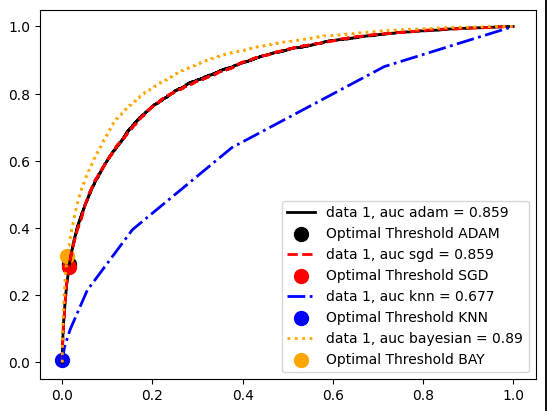
\includegraphics[width=0.25\textwidth]{AUC_santander.png}}
\caption{Curva ROC da base de dados Santander.}
\label{fig}
\end{figure}

\vspace{25pt}

Como analisado anteriormente, os pontos destacados contém o valor do threshold que resultam em uma melhor acurácia do modelo, e serão utilizados como limiar no modelo final do classificador.

\vspace{10pt}

\begin{table}[htbp]
\caption{Resultados dos classificadores para a base de dados do Santander.}
\begin{center}
\begin{tabular}{|c|c|c|c|c|c|}
\hline
\textbf{Classifier} & \textbf{\textit{acc\_cv}} & \textbf{\textit{acc\_test}} & \textbf{\textit{acc\_kaggle}} & \textbf{\textit{t\_train}} & \textbf{\textit{t\_test}} \\
\hline
KNN & (89.0 \(\pm\) 0.1)\% & 88.9\% & 50\% & 16 m & 26s \\
\hline
Naive Bayes & (92.12 \(\pm\) 0.01)\% & 92\% & 68\% & 57 s & 1.31 s \\
\hline
MLP\&SGD & (91.32 \(\pm\) 0.05)\% & \% & 63.9\% &  50 m & 28.1 s \\
\hline
MLP\&ADAM & (91.38 \(\pm\) 0.01)\% & 85\% & 64.75\% & 40 m & 25.1 s \\
\hline
\multicolumn{6}{l}{$^{\mathrm{a}}$ Sample of a Table footnote.}
\end{tabular}
\label{tab1}
\end{center}
\end{table}

Observando a tabela, é possível notar claramente que o classificador ingênuo de Bayes é o algoritmo que melhor se ajusta à base de dados Santander. Este classificador obteve a melhor acurácia, uma maior área sob a curva ROC e necessitou de consideravelmente menos tempo para treino e teste. A base de dados contém várias características que contribuem para essa boa performance do modelo, como atributos independentes e que seguem uma distribuição normal.

O algoritmo KNN apresentou, proporcionalmente, o maior aumento no tempo de teste. Isso ocorre porque a base de dados possui 200.000 linhas e, portanto, para cada amostra a ser classificada, é necessário calcular 200.000 distâncias, o que exige um elevado custo computacional. Sua acurácia foi relativamente baixa, pois o GridSearch para esse modelo variava no intervalo [1, 50], resultando em uma desproporção entre o número de vizinhos K e o conjunto de amostras de treinamento. 

\begin{figure}[htbp]
\centerline{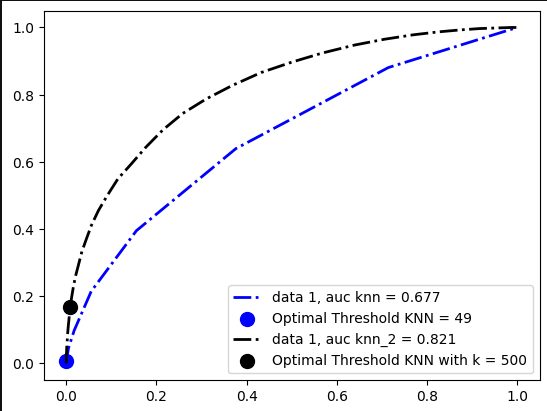
\includegraphics[width=0.25\textwidth]{knn_diff.png}}
\caption{Curva ROC com diferentes valores de k.}
\label{fig}
\end{figure}

Como pode ser observado na imagem acima, ao aumentar o valor de K, foi possível obter uma melhora significativa na acurácia do modelo e na área sob a curva ROC.

As redes neurais perceptron de múltiplas camadas (MLP) demoraram consideravelmente mais tempo para treinar do que todos os outros algoritmos mencionados acima, devido à sua maior complexidade e custo computacional. Considerando ambos os otimizadores, tanto o ADAM quanto o SGD, a rede continha 2 camadas, com 2 neurônios na primeira camada e 1 neurônio na segunda. Redes mais complexas e com mais camadas poderiam ter um desempenho melhor em uma base de dados grande e extensa como essa, mas também exigiriam um alto poder de processamento e tempo para processar todos esses dados.

\section{Conclusion}

Ao realizar o experimento com os modelos de machine learning KNN, Naive Bayes, e redes neurais MLP utilizando os otimizadores ADAM e gradiente estocástico SGD, em duas bases de dados distintas, algumas conclusões importantes emergem dos resultados obtidos. Primeiramente, é evidente que as redes neurais de múltiplas camadas são computacionalmente intensivas, requerendo considerável tempo e energia em comparação aos modelos outros modelos, que são mais simples. Para mitigar esse problema, diferentes otimizadores podem ser empregados para acelerar a convergência dos parâmetros da rede em direção ao ponto de mínimo da função de custo.

O otimizador ADAM, com a sua taxa de aprendizado adaptativa \(\alpha\) e termo de momentum, demonstrou uma convergência mais rápida em comparação ao gradiente estocástico SGD, que atualiza seus parâmetros de forma estocástica com base em entradas aleatórias.

Outro ponto de destaque é o desempenho do classificador ingênuo de Bayes (Naive Bayes). Este modelo, que assume a independência entre as variáveis de entrada, exibiu uma acurácia inferior aos demais na base de dados Titanic. No entanto, ele demandou significativamente menos tempo para treinamento e teste. Em contrapartida, na base de dados do Santander, o Naive Bayes mostrou um desempenho relativamente robusto. A disparidade de desempenho do Naive Bayes entre essas duas bases pode ser atribuída a várias razões, incluindo a representatividade dos dados. É possível que a base de dados Titanic possua características menos representativas em comparação à base do Santander, o que poderia levar o classificador a cometer mais erros de classificação.

Por fim, é importante comentar sobre o tempo gasto na execução do algoritmo GridSearch, visto que as redes neurais de múltiplas camadas demandaram um tempo consideravelmente alto para encontrar a melhor combinação de hiperparâmetros. Esse tempo pode variar conforme o tamanho da base de dados e a capacidade dos componentes que a processam. No entanto, esse tempo pode ser reduzido utilizando máquinas com processadores mais modernos e rápidos, ou processadores dedicados a acelerar esse tipo de serviço, como as recentes Neural Processing Units (NPUs).

\section{Anexo dos códigos, tanto para o Titanic quanto para o Santander : }
Os links para os códigos podem ser encontrados nos seguintes URLs:
\begin{itemize}
    \item \href{https://www.kaggle.com/code/arthurfelipereis/titan-code}
    \item \href{https://www.kaggle.com/code/arthurfelipereis/santander-code}
\end{itemize}


\begin{thebibliography}{00}
\bibitem{b1} Braga, A P, Carvalho, A P L e Ludermir, T B (2007). Redes neurais artificiais: teoria e aplicações. LTC, Livros Técnicos e Científicos.
\bibitem{b2} F. -J. Yang, "An Implementation of Naive Bayes Classifier," 2018 International Conference on Computational Science and Computational Intelligence (CSCI), Las Vegas, NV, USA, 2018, pp. 301-306
\bibitem{b3} I. Fadil, M. A. Helmiawan, F. Supriadi, A. Saeppani, Y. Sofiyan and A. Guntara, "Waste Classifier using Naive Bayes Algorithm," 2022 10th International Conference on Cyber and IT Service Management (CITSM), Yogyakarta, Indonesia, 2022, pp. 1-5, doi: 10.1109/CITSM56380.2022.9935894.
\bibitem{b4} REDDI, Sashank J.; HE, Tao; KAISER, Lukasz; KUMAR, Sanjiv. An overview of gradient descent optimization algorithms
\bibitem{b5} J. Qin, L. Chen, Y. Liu, C. Liu, C. Feng, and B. Chen, “A Machine learning Methodology for diagnosing chronic kidney disease,” IEEE Access, vol. 8, pp. 20991–21002, Jan. 2020.
\bibitem{b6} Castro CL, Braga AP. Optimization of the area under the ROC curve. 2008 10th Brazilian Symposium on Neural Networks, Salvador, Brazil; 2008. p. 141–146. https://doi.org/10. 1109/SBRN.2008.25.
\bibitem{b7} Bradley AP. The use of the area under the ROC curve in the evaluation of machine learning algorithms. Pattern Recogn. 1997; 30:1145–59.
\bibitem{b8} P. K. Diederik and B. A. Jimmy, “Adam: a method for stochastic optimization,” 2014, https://arxiv.org/abs/1412.6980.
\bibitem{b9} T. Badriyah, N. Sakinah, I. Syarif, and D. R. Syarif, “Machine learning algorithm for stroke disease classification,” in Proc. of ICECCE, 2020
\vspace{12pt}
\end{document}
